% OPERA Pit-Wall Screen: preprint.
% Every number in this file comes from numbers.tex and the tab_*.tex tables, which
% code/09_preprint_numbers.py writes from the pipeline's result files. Do not type numbers here.
\documentclass[aps,prd,twocolumn,superscriptaddress,nofootinbib,floatfix,preprintnumbers,10pt]{revtex4-2}
\usepackage[T1]{fontenc}
\usepackage{courier}
\usepackage{mathpazo}
\usepackage{amsmath,amssymb,bm}
\usepackage{graphicx}
\usepackage{booktabs}
\usepackage{xcolor}
\usepackage{tikz}
\usetikzlibrary{positioning,arrows.meta,fit}
\usepackage{hyperref}
\hypersetup{colorlinks=true,linkcolor=red!70!black,citecolor=blue!70!black,urlcolor=blue!60!black}
\usepackage{orcidlink}
% Generated by code/09_preprint_numbers.py from the result files. Do not edit by hand.
\newcommand{\AliasNisar}{181}
\newcommand{\AliasRatio}{4.3}
\newcommand{\AliasSix}{84}
\newcommand{\AliasTwelve}{42}
\newcommand{\AliasTwentyFour}{21}
\newcommand{\Chance}{10\%}
\newcommand{\ChanceAtmEight}{2\%}
\newcommand{\ChanceAtmEightCor}{0\%}
\newcommand{\ChanceAtmTwo}{57\%}
\newcommand{\ChanceAtmTwoCor}{0\%}
\newcommand{\ChanceCor}{0\%}
\newcommand{\ChanceSix}{62\%}
\newcommand{\ChanceSixCor}{0\%}
\newcommand{\ChanceWinFourEight}{5\%}
\newcommand{\ChanceWinFourEightCor}{0\%}
\newcommand{\ChanceWinOneTwoZero}{65\%}
\newcommand{\ChanceWinOneTwoZeroCor}{0\%}
\newcommand{\ChanceWinSevenTwo}{10\%}
\newcommand{\ChanceWinSevenTwoCor}{0\%}
\newcommand{\DEastAscMid}{0.11}
\newcommand{\DEastDescMid}{0.98}
\newcommand{\ExampleLead}{20}
\newcommand{\ExampleNorthAlerts}{1}
\newcommand{\ExampleSouthAlerts}{3}
\newcommand{\FA}{0.20}
\newcommand{\FAAtmEight}{0.07}
\newcommand{\FAAtmEightCor}{0.01}
\newcommand{\FAAtmTwo}{1.21}
\newcommand{\FAAtmTwoCor}{0.00}
\newcommand{\FACor}{0.00}
\newcommand{\FASix}{1.28}
\newcommand{\FASixCor}{0.01}
\newcommand{\FAWallYears}{359}
\newcommand{\FAWinFourEight}{0.03}
\newcommand{\FAWinFourEightCor}{0.00}
\newcommand{\FAWinOneTwoZero}{1.42}
\newcommand{\FAWinOneTwoZeroCor}{0.00}
\newcommand{\FAWinSevenTwo}{0.16}
\newcommand{\FAWinSevenTwoCor}{0.00}
\newcommand{\GeoBlindEitherFiftyFive}{34\%}
\newcommand{\GeoBlindEitherFortyFive}{0\%}
\newcommand{\GeoBlindEitherThirtyFive}{0\%}
\newcommand{\GeoBlindSingleFiftyFive}{48\%}
\newcommand{\GeoBlindSingleFortyFive}{21\%}
\newcommand{\GeoBlindSingleThirtyFive}{34\%}
\newcommand{\GeoLaySingleFiftyFive}{31\%}
\newcommand{\GeoLaySingleFortyFive}{20\%}
\newcommand{\GeoLaySingleThirtyFive}{0\%}
\newcommand{\GeoSensEitherFiftyFive}{66\%}
\newcommand{\GeoSensEitherFortyFive}{97\%}
\newcommand{\GeoSensEitherThirtyFive}{90\%}
\newcommand{\GeoSensSingleFiftyFive}{46\%}
\newcommand{\GeoSensSingleFortyFive}{54\%}
\newcommand{\GeoSensSingleThirtyFive}{46\%}
\newcommand{\GeoShaSingleFiftyFive}{17\%}
\newcommand{\GeoShaSingleFortyFive}{0\%}
\newcommand{\GeoShaSingleThirtyFive}{0\%}
\newcommand{\GeoVisEitherFiftyFive}{66\%}
\newcommand{\GeoVisEitherFortyFive}{100\%}
\newcommand{\GeoVisEitherThirtyFive}{100\%}
\newcommand{\GeoVisSingleFiftyFive}{52\%}
\newcommand{\GeoVisSingleFortyFive}{80\%}
\newcommand{\GeoVisSingleThirtyFive}{100\%}
\newcommand{\HiddenPx}{0}
\newcommand{\KChanceFour}{0\%}
\newcommand{\KChanceFourCor}{0\%}
\newcommand{\KChanceThree}{10\%}
\newcommand{\KChanceThreeCor}{0\%}
\newcommand{\KChanceThreeHalf}{5\%}
\newcommand{\KChanceThreeHalfCor}{0\%}
\newcommand{\KChanceTwo}{68\%}
\newcommand{\KChanceTwoCor}{12\%}
\newcommand{\KChanceTwoHalf}{42\%}
\newcommand{\KChanceTwoHalfCor}{0\%}
\newcommand{\KFAFour}{0.00}
\newcommand{\KFAFourCor}{0.00}
\newcommand{\KFAThree}{0.20}
\newcommand{\KFAThreeCor}{0.00}
\newcommand{\KFAThreeHalf}{0.03}
\newcommand{\KFAThreeHalfCor}{0.00}
\newcommand{\KFATwo}{1.73}
\newcommand{\KFATwoCor}{0.28}
\newcommand{\KFATwoHalf}{0.68}
\newcommand{\KFATwoHalfCor}{0.04}
\newcommand{\KNGrid}{480}
\newcommand{\KPreThree}{12}
\newcommand{\KPreTwo}{112}
\newcommand{\KWFour}{37\%}
\newcommand{\KWFourCor}{41\%}
\newcommand{\KWThree}{55\%}
\newcommand{\KWThreeCor}{53\%}
\newcommand{\KWThreeHalf}{44\%}
\newcommand{\KWThreeHalfCor}{47\%}
\newcommand{\KWTwo}{86\%}
\newcommand{\KWTwoCor}{75\%}
\newcommand{\KWTwoHalf}{74\%}
\newcommand{\KWTwoHalfCor}{63\%}
\newcommand{\KWarnedThree}{265}
\newcommand{\KWarnedTwo}{412}
\newcommand{\LFourOneTwenty}{56}
\newcommand{\LFourOneTwentyCor}{68}
\newcommand{\LFourSixty}{20}
\newcommand{\LFourSixtyCor}{20}
\newcommand{\LFourTwoForty}{128}
\newcommand{\LFourTwoFortyCor}{122}
\newcommand{\LHalfOneTwenty}{68}
\newcommand{\LHalfOneTwentyCor}{--}
\newcommand{\LOneOneTwenty}{14}
\newcommand{\LOneOneTwentyCor}{20}
\newcommand{\LOneTwoForty}{20}
\newcommand{\LOneTwoFortyCor}{20}
\newcommand{\LSix}{56}
\newcommand{\LSixCor}{23}
\newcommand{\LTwoOneTwenty}{20}
\newcommand{\LTwoOneTwentyCor}{32}
\newcommand{\LTwoSixty}{8}
\newcommand{\LTwoSixtyCor}{8}
\newcommand{\LamC}{5.55}
\newcommand{\LamL}{23.8}
\newcommand{\MissFourSixty}{5}
\newcommand{\MissFourSixtyCor}{2}
\newcommand{\MissTwoAll}{0}
\newcommand{\NReal}{2{,}560}
\newcommand{\NRealArm}{1{,}280}
\newcommand{\NoiseAtmEight}{6.8}
\newcommand{\NoiseAtmTwo}{2.0}
\newcommand{\NoiseDefault}{3.5}
\newcommand{\NoiseSix}{2.4}
\newcommand{\NoiseWinFourEight}{6.6}
\newcommand{\NoiseWinOneTwoZero}{1.6}
\newcommand{\NoiseWinSevenTwo}{3.6}
\newcommand{\NullFour}{2.46}
\newcommand{\NullFourCor}{0.00}
\newcommand{\NullOne}{0.20}
\newcommand{\NullOneCor}{0.00}
\newcommand{\NullTwo}{1.52}
\newcommand{\NullTwoCor}{0.00}
\newcommand{\NullUnmatchedCor}{0}
\newcommand{\NullWallYearsCor}{1{,}435}
\newcommand{\NullZero}{0.02}
\newcommand{\NullZeroCor}{0.00}
\newcommand{\PBuffer}{150}
\newcommand{\PCluster}{3}
\newcommand{\PClusterArea}{2{,}700}
\newcommand{\PCoh}{0.6}
\newcommand{\PCohFrac}{50\%}
\newcommand{\PFloor}{2}
\newcommand{\PGrace}{30}
\newcommand{\PK}{3}
\newcommand{\PLead}{180}
\newcommand{\PMinObs}{4}
\newcommand{\PPersist}{2}
\newcommand{\PStableGap}{500}
\newcommand{\PStableKeep}{50\%}
\newcommand{\PStableMin}{20}
\newcommand{\PStableSlope}{10}
\newcommand{\PStableWidth}{2{,}000}
\newcommand{\PWallSlope}{25}
\newcommand{\PWindow}{72}
\newcommand{\QuarterC}{1.39}
\newcommand{\QuarterL}{5.96}
\newcommand{\SagaFar}{0.39}
\newcommand{\SagaMid}{0.46}
\newcommand{\SagaNear}{0.54}
\newcommand{\Seeds}{40}
\newcommand{\WAtmEight}{2\%}
\newcommand{\WAtmEightCor}{5\%}
\newcommand{\WAtmTwo}{95\%}
\newcommand{\WAtmTwoCor}{92\%}
\newcommand{\WFourOneTwenty}{100\%}
\newcommand{\WFourOneTwentyCor}{100\%}
\newcommand{\WFourSixty}{88\%}
\newcommand{\WFourSixtyCor}{95\%}
\newcommand{\WFourTwoForty}{100\%}
\newcommand{\WFourTwoFortyCor}{100\%}
\newcommand{\WHalfOneTwenty}{12\%}
\newcommand{\WHalfOneTwentyCor}{0\%}
\newcommand{\WOneOneTwenty}{30\%}
\newcommand{\WOneOneTwentyCor}{30\%}
\newcommand{\WOneTwoForty}{32\%}
\newcommand{\WOneTwoFortyCor}{30\%}
\newcommand{\WSix}{92\%}
\newcommand{\WSixCor}{95\%}
\newcommand{\WTwoOneTwenty}{85\%}
\newcommand{\WTwoOneTwentyCor}{92\%}
\newcommand{\WTwoSixty}{75\%}
\newcommand{\WTwoSixtyCor}{75\%}
\newcommand{\WWinFourEight}{5\%}
\newcommand{\WWinFourEightCor}{5\%}
\newcommand{\WWinOneTwoZero}{85\%}
\newcommand{\WWinOneTwoZeroCor}{85\%}
\newcommand{\WWinSevenTwo}{25\%}
\newcommand{\WWinSevenTwoCor}{25\%}

\newcommand{\vhat}[1]{\hat{\bm{#1}}}
\renewcommand{\arraystretch}{1.12}

\begin{document}
% Generated by code/09_preprint_numbers.py. Draft marker until the author verifies (--final removes it).


\title{Can NASA's open OPERA InSAR product screen open-pit walls?\\ Geometric limits, simulation benchmarks, and a reproducible pipeline for a two-site pilot}

\author{Lukman Alabede\,\orcidlink{0009-0008-7769-7455}}
\email{lukmanademola081@gmail.com}
\affiliation{Independent Researcher}
\author{Kayode Komolafe\,\orcidlink{0000-0001-8279-821X}}
\email{komolafe@mines.edu}
\affiliation{Mining Engineering Department, Colorado School of Mines, Golden, Colorado, USA}

\begin{abstract}
Open-pit wall failures endanger workers and interrupt production, yet the monitoring records that large operators keep are private, and there is no public evidence on whether free satellite data can screen walls that are not otherwise watched. Since 2025 NASA's OPERA project has distributed DISP-S1, a standardized line-of-sight (LOS) displacement product from Sentinel-1 at 30~m posting over North America from mid-2016. We present an open, tested pipeline that turns DISP-S1 into wall-by-wall alerts and scores them against documented wall failures, and we establish, before any real-data result, what the product can and cannot see. Geometric analysis shows that a single Sentinel-1 pass records at least half of a downslope slide on only \GeoSensSingleFortyFive{} of wall facing directions for $45^\circ$ walls (\GeoSensEitherFortyFive{} with both passes), and that walls steeper than about $55^\circ$ fall increasingly into layover or shadow. Phase aliasing caps recordable LOS motion at about \AliasTwelve{}~cm/yr at a 12-day revisit, against \AliasNisar{}~cm/yr for NISAR L-band. In \NReal{} simulated pits, the default alert rule warned before failure in \WTwoOneTwenty{} of scenes with 2~cm-scale accelerating creep (median lead \LTwoOneTwenty{}~days) at a chance rate of \Chance{} and \FA{} alerts without an event per wall-year, while 0.5~cm-scale creep could not be distinguished from chance. The simulations also expose a failure mode: atmospheric delay that tracks pit depth dominates false alerts whenever random noise is low, so a longer velocity window or a 6-day revisit raises the chance warning rate to \ChanceWinOneTwoZero{} and \ChanceSix{}. A per-date elevation regression removed these alerts in simulation (\NullUnmatchedCor{} in \NullWallYearsCor{} no-creep wall-years) and kept or improved real warnings: \WTwoOneTwentyCor{} for 2~cm-scale creep (median lead \LTwoOneTwentyCor{}~days), and \WSixCor{} for 1~cm-scale creep with a 6-day revisit. We map the predictions onto two documented failures, the 2022 Continental Pit (Montana) and 2023 Saga Pit (Nevada) events, as testable expectations for the pilot. All code, tests and provenance are public.
\smallskip

\noindent\textbf{Keywords:} InSAR, OPERA DISP-S1, Sentinel-1, open-pit mining, slope stability, early warning, NISAR
\end{abstract}

\maketitle

%=====================================================================
\section{Introduction}
%=====================================================================

Large open pits are among the deepest excavations people make, and their walls are designed with explicit, accepted probabilities of failure~\cite{ReadStacey2009}. When a wall moves more than expected, the consequences range from lost benches to events such as the 2013 Manefay slide at Bingham Canyon, Utah, which moved about 145 million tonnes of rock and waste~\cite{Pankow2014,Gaida2019}. Operators manage this risk with layered monitoring: survey prisms, ground-based radar, and increasingly commercial satellite interferometric synthetic aperture radar (InSAR). The interpretation of the resulting displacement records rests on a long empirical tradition in which slopes approaching failure accelerate, so that inverse velocity falls roughly linearly toward the time of collapse~\cite{Fukuzono1985,Voight1988,Dick2015,Carla2017}.

Satellite InSAR measures ground displacement along the radar line of sight (LOS) from the phase difference between repeat images, with millimetre sensitivity over areas of thousands of square kilometres~\cite{Massonnet1998,Rosen2000,Hanssen2001}. Multi-temporal methods that exploit persistent and distributed scatterers made it a standard tool for unstable slopes~\cite{Ferretti2001,Berardino2002,Colesanti2006,Wasowski2014}. Retrospective studies show that Sentinel-1 data recorded accelerating precursors before large slope failures, including an open-pit slope~\cite{Carla2019,Intrieri2018}. At Bingham Canyon, reprocessed historical InSAR revealed movement for years before the Manefay slide~\cite{Gaida2019}. A back-analysis of two wall failures at the Bald Mountain Mine, Nevada, found Sentinel-1 precursory motion months before the January 2023 failure of the Saga Pit north wall~\cite{Bourgeois2024}.

These studies share two features that limit their public value. They relied on custom or commercial processing, and the records of the many operators who monitor walls privately are not available to regulators, smaller mines, communities or researchers. The question a state inspector or a small operator would ask, whether free government data can flag a wall that deserves attention, and where it is blind, has no public, reproducible answer.

Two developments make that question answerable. First, NASA's Observational Products for End-Users from Remote Sensing Analysis (OPERA) project released DISP-S1 in 2025: LOS displacement from Sentinel-1, produced by sequential phase linking on compressed single-look complex images, posted at 30~m on a UTM grid, and covering the United States and much of North America from mid-2016~\cite{OperaDISP,OperaRelease2025,OperaATBD2025,Staniewicz2025,Staniewicz2024}. Second, the NASA--ISRO NISAR mission, launched on 30 July 2025, adds L-band observations on a 12-day cycle~\cite{ISRONISAR}, and OPERA has announced a corresponding displacement product.

This paper makes four contributions. (i) A reproducible, tested pipeline that turns DISP-S1 granules into wall-by-wall alerts, scores them against documented failures, and reports where the product cannot see (Sec.~\ref{sec:methods}). (ii) A closed-form analysis of which wall orientations and slopes Sentinel-1 can observe, and how much of a downslope slide it records (Sec.~\ref{sec:geom}). (iii) A simulation study of \NReal{} synthetic pits that quantifies detection, lead time, and false alerts as functions of creep magnitude, alert threshold, velocity window, revisit and atmosphere. The study identifies depth-correlated atmospheric delay as the dominant source of false alerts and tests a correction (Sec.~\ref{sec:sim}). (iv) Explicit, testable expectations for a two-site pilot at documented failures in Montana and Nevada, stated before the real data are analysed (Sec.~\ref{sec:discussion}).

The remainder is organized as follows. Section~\ref{sec:data} describes the data and the pilot sites. Section~\ref{sec:methods} gives the method. Section~\ref{sec:results} reports the geometric and simulation results. Section~\ref{sec:discussion} discusses what they imply for the pilot and for public screening. Section~\ref{sec:limits} lists limitations, and Section~\ref{sec:conclusions} concludes.

%=====================================================================
\section{Data and study design}\label{sec:data}
%=====================================================================

\subsection{The OPERA DISP-S1 product}

DISP-S1 is distributed by the Alaska Satellite Facility (ASF) archive as HDF5 granules, one per frame and acquisition~\cite{OperaDISP}. Frames nominally contain 27 Sentinel-1 bursts, overlap their along-track neighbours by one burst, and are posted at $30\times30$~m on the UTM zone of the frame centre~\cite{OperaATBD2025}. Persistent scatterers are processed at single look. Distributed scatterers are phase-linked over statistically homogeneous neighbourhoods, and each mini-stack of typically 15 to 30 acquisitions is compressed into one complex image that is carried into the next mini-stack~\cite{OperaATBD2025,Staniewicz2025}. Each granule reports displacement relative to a reference date stored in its metadata, and users concatenate consecutive granules to obtain a full series~\cite{OperaATBD2025}. Positive values denote apparent motion toward the satellite~\cite{OperaATBD2025}. The primary displacement layer is unfiltered, and ionospheric and solid-Earth-tide corrections are provided as separate layers rather than applied~\cite{OperaATBD2025}. No tropospheric correction is applied. This matters below. Each granule also carries a temporal-coherence layer and a recommended mask. A companion product, DISP-S1-STATIC, provides per-frame LOS unit vectors and a layover/shadow mask~\cite{OperaStatic}.

\subsection{Acquisition geometry and revisit}

Sentinel-1 is a right-looking C-band radar ($\lambda=\LamC$~cm) in a sun-synchronous orbit, imaging in Interferometric Wide swath mode at incidence angles of roughly $29^\circ$ to $46^\circ$~\cite{Torres2012}. Over most land areas the archive is sampled every 12 days. A 6-day sampling is available only where both satellites of the constellation were tasked~\cite{ASFS1}. Sentinel-1B stopped acquiring on 23 December 2021, and Sentinel-1C, launched on 5 December 2024, replaced it~\cite{ASFS1}. Both pilot failures therefore fall in a single-satellite period with a 12-day revisit at best, which bounds both the velocity that can be recorded without phase ambiguity (Sec.~\ref{sec:alias}) and the achievable lead time.

\subsection{Elevation model}

Wall outlines and candidate stable ground are delineated from the Copernicus DEM GLO-30, a 30~m global surface model distributed through the Registry of Open Data on AWS~\cite{CopDEM}. Its radar acquisitions date from about 2011 to 2015, so walls cut or pushed back after that are missing or misplaced. The pipeline therefore produces a preview map for the analyst, and any hand-drawn outline overrides the automatic one.

\subsection{Pilot sites and documented failures}

The pilot uses two open pits with a dated, publicly documented wall failure inside the DISP-S1 record (Table~\ref{tab:events}). Sites operated by the first author's employer are excluded by a filter enforced on every run. The filter matches each site's operator, name and identifier against a list kept outside the public repository.

\emph{Continental Pit, Butte, Montana.} The Montana Department of Environmental Quality reported that about one million tons of rock were displaced along a series of benches in the central D East highwall during the night of 1 November 2022~\cite{MTDEQ2022}. The operator had observed instability and discussed it with the regulator in late September and October 2022, and the failure was ``predicted by the pit monitoring system''~\cite{MTDEQ2022}. Measurable precursory motion is therefore known to have existed.

\emph{Saga Pit, Bald Mountain Mine, Nevada.} The north wall failed on 20 January 2023. A back-analysis of commercially processed Sentinel-1 data from two descending tracks found crest movement from July 2022 and acceleration from November 2022. Images in the final weeks were excluded because of heavy snow~\cite{Bourgeois2024}. This site allows a direct test of whether the free standardized product records what custom processing of the same satellites recorded.

\begin{table*}[t]
\caption{Documented wall failures used in the pilot. Event dates and descriptions are taken from the cited sources; neither source gives coordinates on the wall.}
\label{tab:events}
\begin{ruledtabular}
\begin{tabular}{llllp{7.2cm}}
Site & Wall & Date & Size & Evidence of precursory movement \\
\hline
Continental Pit, MT & D East highwall & 2022-11-01 & $\sim$1 Mt & Instability observed and discussed with the regulator, late Sep.--Oct.\ 2022; failure predicted by the pit monitoring system~\cite{MTDEQ2022} \\
Saga Pit, Bald Mountain, NV & North wall & 2023-01-20 & not reported & Commercial Sentinel-1 InSAR: crest movement from July 2022, acceleration from Nov.\ 2022; final pre-failure images lost to snow~\cite{Bourgeois2024} \\
\end{tabular}
\end{ruledtabular}
\end{table*}

%=====================================================================
\section{Methods}\label{sec:methods}
%=====================================================================

Figure~\ref{fig:pipeline} summarizes the pipeline~\cite{Alabede2026}. Every threshold is a named parameter (Table~\ref{tab:params}), every number in this paper is read from files the pipeline writes, and the software is tested against synthetic pits with known answers.

\begin{figure*}[t]
\centering
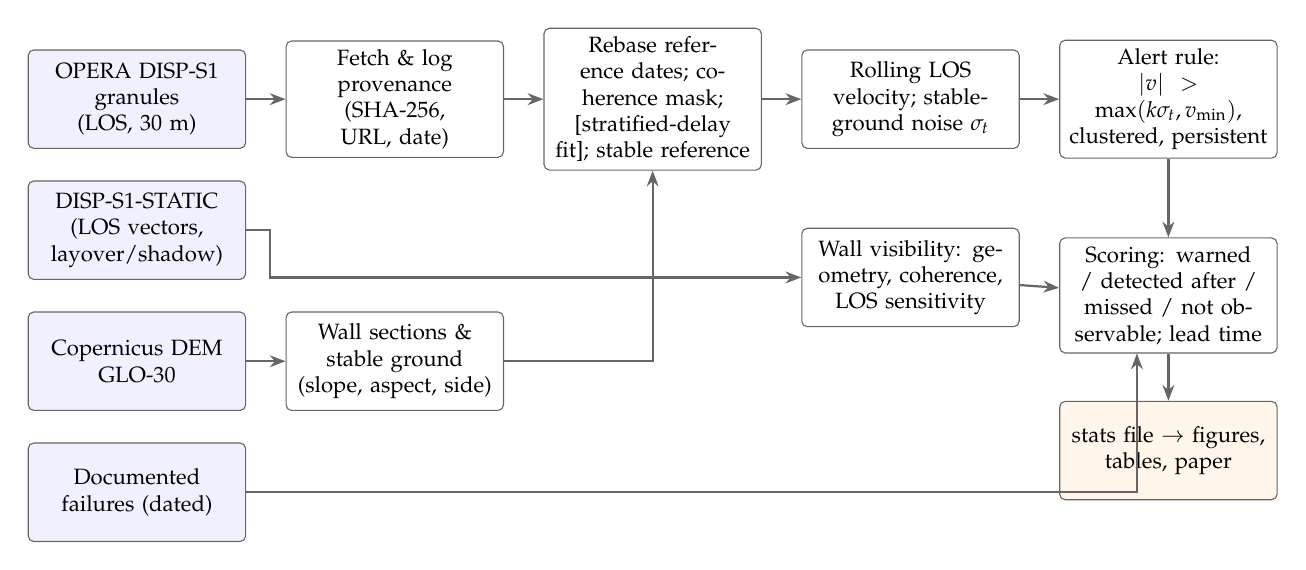
\begin{tikzpicture}[
  node distance=4mm and 5mm,
  box/.style={draw=black!60, rounded corners=2pt, align=center, font=\footnotesize, inner sep=3pt, text width=2.55cm, minimum height=1.25cm, fill=white},
  inbox/.style={box, fill=blue!6},
  outbox/.style={box, fill=orange!8},
  arr/.style={-{Stealth[length=2mm]}, thick, black!60}]
\node[inbox] (disp) {OPERA DISP-S1\\granules (LOS, 30~m)};
\node[inbox, below=of disp] (static) {DISP-S1-STATIC\\(LOS vectors, layover/shadow)};
\node[inbox, below=of static] (dem) {Copernicus DEM\\GLO-30};
\node[inbox, below=of dem] (ev) {Documented\\failures (dated)};
\node[box, right=of disp] (fetch) {Fetch \& log provenance\\(SHA-256, URL, date)};
\node[box, right=of dem] (walls) {Wall sections \&\\stable ground\\(slope, aspect, side)};
\node[box, right=of fetch] (stack) {Rebase reference dates; coherence mask; [stratified-delay fit]; stable reference};
\node[box, right=of stack] (vel) {Rolling LOS velocity; stable-ground noise $\sigma_t$};
\node[box, right=of vel] (alert) {Alert rule:\\$|v|>\max(k\sigma_t,v_{\min})$, clustered, persistent};
\node[box, below=of alert, yshift=-6mm] (valid) {Scoring: warned / detected after / missed / not observable; lead time};
\node[box, below=of vel, yshift=-6mm] (vis) {Wall visibility: geometry, coherence, LOS sensitivity};
\node[outbox, below=of valid, yshift=-2mm] (outs) {stats file $\rightarrow$ figures, tables, paper};
\draw[arr] (disp) -- (fetch); \draw[arr] (fetch) -- (stack);
\draw[arr] (static.east) -- ++(3mm,0) |- (vis.west);
\draw[arr] (dem) -- (walls); \draw[arr] (walls.east) -| (stack.south);
\draw[arr] (stack) -- (vel); \draw[arr] (vel) -- (alert); \draw[arr] (alert) -- (valid);
\draw[arr] (ev.east) -| ([xshift=-4mm]valid.south) ;
\draw[arr] (vis) -- (valid); \draw[arr] (valid) -- (outs);
\end{tikzpicture}
\caption{The OPERA Pit-Wall Screen pipeline. Blue: public inputs. The bracketed stratified-delay fit is optional and evaluated in Sec.~\ref{sec:sim}. Each step is a numbered script, and every number in the outputs is written to one stats file that the figures, tables and this paper read.}
\label{fig:pipeline}
\end{figure*}

\subsection{Time-series reconstruction}

For a frame, let granule $g$ report displacement $d_g(\bm{x}) = D(s_g,\bm{x}) - D(r_g,\bm{x})$ between its reference date $r_g$ and secondary date $s_g$. Sorting granules by $s_g$ and setting $D(t_0)=0$ at the earliest reference date, each granule is placed by
\begin{equation}
D(s_g,\bm{x}) = D(r_g,\bm{x}) + d_g(\bm{x}),
\label{eq:rebase}
\end{equation}
which requires $D(r_g)$ to be known, i.e.\ $r_g = t_0$ or $r_g$ is the secondary date of an earlier granule. When it is not, because of a gap in the archive, a new segment begins and the break is recorded. Velocities are never fitted across a segment break. Equation~(\ref{eq:rebase}) reduces to the identity when all granules share one reference date, so it is valid for either reference convention. Only the window around the site is read from each granule.

\subsection{Quality masking and stable-ground reference}

A pixel is valid on date $t$ when its temporal coherence is at least $\gamma_{\min}=\PCoh$, it is flagged usable by the recommended mask, and it is not water. Each date is then referenced to ground judged stable,
\begin{equation}
\tilde{D}(t,\bm{x}) = D(t,\bm{x}) - \operatorname*{med}_{\bm{x}'\in\mathcal{S}_t} D(t,\bm{x}'),
\label{eq:ref}
\end{equation}
where $\mathcal{S}_t$ is the set of valid stable pixels. Dates with fewer than \PStableMin{} such pixels are discarded. Candidate stable ground is gently sloping terrain (slope at most $\PStableSlope^\circ$) in a ring \PStableGap{} to \PStableWidth{}~m beyond the pit. Because candidates can include settling waste dumps or tailings, only the \PStableKeep{} of candidates with the smallest whole-record trend are kept. This step uses neither the walls nor the failure dates.

\subsection{Optional stratified-delay correction}\label{sec:strat}

Radar delay through a vertically layered troposphere varies with surface height and season~\cite{Doin2009,Hanssen2001}. A pit floor several hundred metres below a stable rim therefore carries a seasonal LOS signal that Eq.~(\ref{eq:ref}) does not remove. As an option, for each date we fit
\begin{equation}
\tilde{D}(t,\bm{x}) = a_t + b_t\, z(\bm{x}) + \varepsilon(t,\bm{x})
\label{eq:strat}
\end{equation}
over all valid pixels by least squares with iterative $3\times$ robust-sigma clipping, and subtract $\hat{b}_t z$. Localized wall motion is a small fraction of the scene and is rejected by the clipping. Its residual leakage into $\hat{b}_t$ is a stated limitation.

\subsection{Automatic wall delineation}

Within a search radius of the pit centre, DEM pixels steeper than $\PWallSlope^\circ$ are wall. Each wall pixel is assigned to one of eight facing directions (aspect sectors) and one of eight sides of the pit (bearing from the centre). The section facing west on the east side, for example, is named \texttt{faces\_W\_E}. Reported wall names are mapped onto these sections, so the D East highwall of the Continental Pit is \texttt{faces\_W\_E}. Where no pit centre is known, as in a multi-pit district, closed depressions more than 40~m below a 2.5~km median-smoothed surface are identified as pits, numbered, and outlined for the analyst. Wall pixels in layover or shadow according to DISP-S1-STATIC are removed before detection.

\subsection{Velocity and noise}

For each date $t$ and pixel, LOS velocity is the least-squares slope over the trailing window $W=\PWindow$~days,
\begin{equation}
v_t(\bm{x}) = \frac{\sum_{\tau\in\mathcal{T}_t} (\tau-\bar\tau)\,\big(\tilde D(\tau,\bm{x})-\bar{D}\big)}{\sum_{\tau\in\mathcal{T}_t} (\tau-\bar\tau)^2},
\label{eq:vel}
\end{equation}
where $\mathcal{T}_t=\{\tau: t-W<\tau\le t,\ \text{same segment, valid}\}$ must contain at least \PMinObs{} dates. The noise level on date $t$ is the robust standard deviation of stable-ground velocities~\cite{Rousseeuw1993},
\begin{equation}
\sigma_t = 1.4826\,\operatorname*{med}_{\bm{x}\in\mathcal{S}_t}\big|v_t(\bm{x}) - \operatorname*{med}_{\mathcal{S}_t} v_t\big|.
\label{eq:sigma}
\end{equation}

\subsection{Alert rule}

A wall pixel exceeds the threshold on date $t$ when
\begin{equation}
|v_t(\bm{x})| > \theta_t = \max\!\big(k\,\sigma_t,\ v_{\min}\big),
\label{eq:thr}
\end{equation}
with $k=\PK$ and $v_{\min}=\PFloor$~cm/yr. Exceeding pixels are grouped into 8-connected patches, and a wall is flagged on date $t$ if any patch has at least $n_{\min}=\PCluster$ pixels (\PClusterArea~m$^2$). An alert is raised on the date when a wall has been flagged on $P=\PPersist$ consecutive dates, and the alert episode lasts while the wall stays flagged.

\subsection{Scoring against documented failures}

Each documented failure at time $t_f$ on wall $w$ is assigned one outcome. It is \emph{not observable} if wall $w$ had fewer than \PMinObs{} usable dates in the $L=\PLead$~days before $t_f$, or if $t_f$ lies outside the data span. It is \emph{warned} if an alert on $w$ was raised before $t_f$ and was still active within $L$ days of it. It is \emph{detected after} if the first alert came on or up to \PGrace{}~days after $t_f$, and \emph{missed} otherwise. A failure whose reported wall cannot yet be placed on the site's wall sections is \emph{unlocated} and excluded from all rates. For warned events the lead time is
\begin{equation}
\ell = t_f - \max\!\big(t_a,\ t_f - L\big),
\label{eq:lead}
\end{equation}
where $t_a$ is the date the alert was raised. With two satellite tracks the better outcome counts. Warning rates carry Wilson 95\% intervals~\cite{Wilson1927},
\begin{equation}
\frac{\hat p + \frac{z^2}{2n} \pm z\sqrt{\frac{\hat p(1-\hat p)}{n}+\frac{z^2}{4n^2}}}{1+\frac{z^2}{n}},\quad z=1.96.
\label{eq:wilson}
\end{equation}
Alerts not followed (or preceded within the grace period) by a documented failure are reported as \emph{alerts without a reported event} rather than false alarms, because public failure records are incomplete.

\begin{table}[t]
\caption{Default settings of the alert rule and scoring. All are configuration values; those marked $^\dagger$ are judgement calls tested in Sec.~\ref{sec:sim}.}
\label{tab:params}
\begin{ruledtabular}
\begin{tabular}{lll}
Quantity & Symbol & Default \\
\hline
Coherence threshold & $\gamma_{\min}$ & \PCoh \\
Velocity window & $W$ & \PWindow{} d$^\dagger$ \\
Minimum dates in window & -- & \PMinObs \\
Threshold multiplier & $k$ & \PK$^\dagger$ \\
Velocity floor & $v_{\min}$ & \PFloor{} cm/yr \\
Minimum patch & $n_{\min}$ & \PCluster{} px \\
Persistence & $P$ & \PPersist{} dates \\
Warning window & $L$ & \PLead{} d \\
Late-detection grace & -- & \PGrace{} d \\
Wall slope threshold & -- & $\PWallSlope^\circ$ \\
Stable-ground slope & -- & $\le\PStableSlope^\circ$ \\
Stratified-delay fit & Eq.~(\ref{eq:strat}) & off$^\dagger$ \\
\end{tabular}
\end{ruledtabular}
\end{table}

\subsection{Observability: LOS sensitivity, layover, shadow and aliasing}\label{sec:obsmethod}

Let $\vhat{l}=(\sin\theta\sin\phi,\ \sin\theta\cos\phi,\ \cos\theta)$ be the unit vector from the ground to the satellite in east--north--up coordinates. Here $\theta$ is the incidence angle and $\phi$ the ground-to-satellite azimuth, equal to the heading minus $90^\circ$ for a right-looking radar. For a wall face of aspect $a$ (the direction it faces) and slope $s$, the downslope unit vector is
\begin{equation}
\vhat{d} = (\sin a\cos s,\ \cos a\cos s,\ -\sin s),
\label{eq:dhat}
\end{equation}
and the fraction of a downslope slide recorded in LOS is $p=\vhat{d}\cdot\vhat{l}$. In the range plane the slope projected on the look direction is
\begin{equation}
\alpha_r = \arctan\!\big[\tan s\,\cos(a-\phi)\big],
\label{eq:alphar}
\end{equation}
with layover when $\alpha_r>\theta$ and shadow when $-\alpha_r>90^\circ-\theta$ (planar approximation). Because the interferometric phase is known only modulo $2\pi$, motion exceeding a quarter wavelength between consecutive acquisitions cannot be recovered unambiguously from neighbouring-date pairs, giving a ceiling
\begin{equation}
v_{\max} = \frac{\lambda}{4\,\Delta t},
\label{eq:alias}
\end{equation}
where $\Delta t$ is the revisit. In practice motion near this limit also decorrelates the signal~\cite{Zebker1992}. We use typical mid-latitude Sentinel-1 headings of $348^\circ$ (ascending) and $192^\circ$ (descending).

\subsection{Simulation design}\label{sec:simdesign}

To measure the alert rule's behaviour where the answer is known, we simulate a $3.6\times3.6$~km scene at 30~m posting containing a 600~m deep conical pit. The pit's walls lie between 450 and 1050~m from its centre (about $45^\circ$) and are split into four walls by facing direction. The west wall is placed in layover. Stable ground is a ring 1.5 to 1.75~km from the centre. A 160~m radius patch on the east wall creeps toward failure at $t_f$ in the inverse-velocity form~\cite{Fukuzono1985,Voight1988}
\begin{equation}
d(t) = -A\ln\!\left(1-\frac{t-t_s}{t_f-t_s+\tau_0}\right),\quad t_s\le t<t_f,
\label{eq:creep}
\end{equation}
so that $1/v = (t_f - t + \tau_0)/A$ falls linearly to $\tau_0/A$ at failure, with $\tau_0=4$~days. Here $A$ is the creep scale and $t_f-t_s$ the precursor duration. The creep patch loses coherence (to 0.2) on any revisit whose motion exceeds $\lambda/4$, and for 36~days after failure. Each date adds three noise terms: a turbulent atmospheric screen (Gaussian-filtered white noise, 750~m correlation scale, standard deviation $\sigma_{\rm atm}=4$~mm by default); a stratified seasonal delay $c\,h(\bm{x})\cos(2\pi t/1\,\mathrm{yr})$ proportional to depth below the rim $h$, with $c=1.2$~mm per 100~m by default; and white pixel noise of 1.5~mm. Granules are cut with a reference date that resets every 15 acquisitions, as in DISP-S1, and pass through the full pipeline. Five studies vary one factor at a time, each with \Seeds{} random realizations per setting: (A) creep scale $A\in\{0.5,1,2,4\}$~cm and precursor duration $\{60,120,240\}$~days; (B) no-creep scenes with $c\in\{0,1.2,2.4,4.8\}$~mm per 100~m; (C) window $W\in\{48,72,120\}$~days; (D) 6-day revisit; (E) $\sigma_{\rm atm}\in\{2,4,8\}$~mm. Every setting is also run on matched no-creep scenes, which give the \emph{chance warning rate}: the probability that a coincidental alert falls in the warning window of a failure with no precursor. Every scene is run with and without the stratified-delay fit of Eq.~(\ref{eq:strat}) on the same random seed, giving \NRealArm{} paired realizations per arm.

\subsection{Reproducibility}

The pipeline consists of numbered scripts with a provenance log (file, size, SHA-256, source URL and access date) for every input. A test suite checks the reconstruction of Eq.~(\ref{eq:rebase}) to $10^{-5}$~m, the UTM transform against a known value, automatic wall naming, the stratified-delay fit, and end-to-end recovery of planted outcomes. A one-button cloud workflow downloads DISP-S1 with the user's free Earthdata credentials and runs every step. Code is released under the MIT licence, and derived data and text under CC BY 4.0~\cite{Alabede2026}.

%=====================================================================
\section{Results}\label{sec:results}
%=====================================================================

\subsection{Which walls Sentinel-1 can see}\label{sec:geom}

Figure~\ref{fig:geometry} shows the recorded fraction $|p|$ of a downslope slide on a $45^\circ$ wall as a function of the direction it faces, at the mid-swath incidence of $39^\circ$. Each pass sees walls facing roughly along its look direction well, with $|p|$ approaching 1 for walls facing away from the satellite. It sees walls facing along the satellite track poorly, where motion is mostly horizontal and perpendicular to the LOS, and only the vertical component is recorded. For a single pass, \GeoSensSingleFortyFive{} of facing directions record at least half of a downslope slide, and \GeoLaySingleFortyFive{} fall in layover (Table~\ref{tab:geom}). Because the two passes look from opposite sides, combining them raises the fraction with $|p|\ge0.5$ to \GeoSensEitherFortyFive{} and leaves no facing direction unobserved. The picture deteriorates quickly with slope. At $55^\circ$ a single pass sees only \GeoVisSingleFiftyFive{} of facing directions (\GeoLaySingleFiftyFive{} layover, \GeoShaSingleFiftyFive{} shadow), and even both passes together see only \GeoVisEitherFiftyFive. The geometry also depends on where the pit falls within the swath (Table~\ref{tab:geom}).

\begin{figure}[t]
\centering
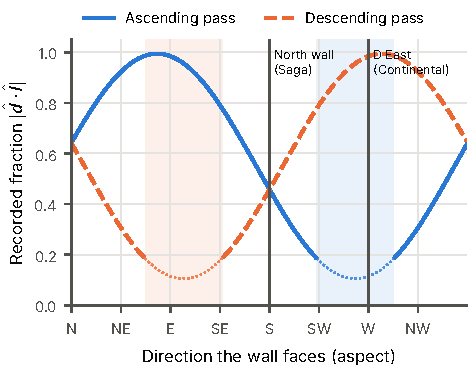
\includegraphics[width=\columnwidth]{fig_geometry.pdf}
\caption{Fraction of a downslope slide recorded in the LOS, $|\vhat{d}\cdot\vhat{l}|$, for a $45^\circ$ wall versus the direction it faces, at $39^\circ$ incidence. Solid and dashed: geometrically visible; dotted with shading: layover for that pass. Vertical lines mark the two pilot walls.}
\label{fig:geometry}
\end{figure}

\begin{table}[t]
\caption{Share of wall facing directions observable by one Sentinel-1 pass (ascending; descending is symmetric) and by either pass, and share recording at least half of a downslope slide ($|p|\ge0.5$).}
\label{tab:geom}
\begin{ruledtabular}
\begin{tabular}{cccccccc}
 & & \multicolumn{4}{c}{One pass} & \multicolumn{2}{c}{Either pass} \\
$\theta$ & $s$ & Vis. & Lay. & Sha. & $|p|\!\ge\!.5$ & Vis. & $|p|\!\ge\!.5$ \\
\hline
% Generated by code/09_preprint_numbers.py. Do not edit by hand.
30 & 35 & 81\% & 19\% & 0\% & 50\% & 100\% & 93\% \\
30 & 45 & 70\% & 30\% & 0\% & 60\% & 100\% & 100\% \\
30 & 55 & 63\% & 37\% & 0\% & 63\% & 100\% & 100\% \\
\hline
39 & 35 & 100\% & 0\% & 0\% & 46\% & 100\% & 90\% \\
39 & 45 & 80\% & 20\% & 0\% & 54\% & 100\% & 97\% \\
39 & 55 & 52\% & 31\% & 17\% & 46\% & 66\% & 66\% \\
\hline
46 & 35 & 100\% & 0\% & 0\% & 45\% & 100\% & 88\% \\
46 & 45 & 91\% & 0\% & 9\% & 41\% & 100\% & 76\% \\
46 & 55 & 49\% & 24\% & 26\% & 29\% & 63\% & 46\% \\

\end{tabular}
\end{ruledtabular}
\end{table}

For the two pilot walls, assuming an overall slope of $45^\circ$, the predictions are specific (Table~\ref{tab:pilotwalls}). The west-facing D East highwall of the Continental Pit lies close to the ascending look direction. At mid-swath it falls in layover for the ascending pass ($|p|=\DEastAscMid$), but is recorded almost fully by the descending pass ($|p|=\DEastDescMid$), moving away from the satellite. At far-range incidence the descending view grazes into shadow. The south-facing Saga north wall faces along the track for both passes, which record the same, mostly vertical, fraction $|p|=\SagaMid$ (\SagaFar{} to \SagaNear{} across the swath). A slide there must be about twice as fast as on a well-aligned wall to cross the same threshold.

\begin{table}[t]
\caption{Predicted LOS fraction $p=\vhat{d}\cdot\vhat{l}$ (negative: away from the satellite) and visibility for the two pilot walls, assuming a $45^\circ$ overall slope, at near, mid and far-range incidence $\theta$.}
\label{tab:pilotwalls}
\begin{ruledtabular}
\begin{tabular}{p{2.3cm}ccc}
Wall & $\theta$ & Ascending & Descending \\
\hline
% Generated by code/09_preprint_numbers.py. Do not edit by hand.
Continental, D East (faces W) & 30 & -0.27 (layover) & -0.96 (visible) \\
 & 39 & -0.11 (layover) & -0.98 (visible) \\
 & 46 & +0.01 (visible) & -0.99 (shadow) \\
\hline
Saga, north wall (faces S) & 30 & -0.54 (visible) & -0.54 (visible) \\
 & 39 & -0.46 (visible) & -0.46 (visible) \\
 & 46 & -0.39 (visible) & -0.39 (visible) \\

\end{tabular}
\end{ruledtabular}
\end{table}

\subsection{Phase-aliasing ceilings}\label{sec:alias}

Table~\ref{tab:alias} evaluates Eq.~(\ref{eq:alias}). At the 12-day revisit typical over North America, Sentinel-1 cannot record more than \QuarterC{}~cm of LOS motion between passes, about \AliasTwelve{}~cm/yr. A wall in the final weeks before failure commonly moves faster than this, so the last stage of acceleration appears in DISP-S1 as lost coherence rather than as large displacement. NISAR's longer L-band wavelength raises the ceiling to about \AliasNisar{}~cm/yr at the same revisit, a factor of \AliasRatio.

\begin{table}[t]
\caption{Maximum LOS motion recordable without phase ambiguity, Eq.~(\ref{eq:alias}).}
\label{tab:alias}
\begin{ruledtabular}
\begin{tabular}{lcccc}
Sensor & $\lambda$ (cm) & $\Delta t$ (d) & cm/revisit & cm/yr \\
\hline
% Generated by code/09_preprint_numbers.py. Do not edit by hand.
Sentinel-1 C-band & 5.55 & 6 & 1.39 & 84 \\
Sentinel-1 C-band & 5.55 & 12 & 1.39 & 42 \\
Sentinel-1 C-band & 5.55 & 24 & 1.39 & 21 \\
NISAR L-band & 23.85 & 12 & 5.96 & 181 \\

\end{tabular}
\end{ruledtabular}
\end{table}

\subsection{Simulation: detection, lead time and chance}\label{sec:sim}

At the default settings the stable-ground noise level was $\sigma_t\approx\NoiseDefault$~cm/yr, so the effective threshold was about three times that. In no-creep scenes, alerts without an event occurred at \FA{} per wall-year. The chance that a coincidental alert falls in the \PLead-day warning window of a failure with no precursor was \Chance. These two figures are consistent: for alerts arriving at rate $\Lambda$ per wall-year, the chance of at least one in a window $L$ is $1-e^{-\Lambda L}$. This is the baseline against which every warning rate below must be read.

Figure~\ref{fig:grid} and Table~\ref{tab:grid} show detection as a function of creep scale and precursor duration. With $A=0.5$~cm the warning rate (\WHalfOneTwenty) does not differ from chance, and the identical results across durations show that these warnings are coincidental. With $A=1$~cm, about \WOneOneTwenty{} of failures were warned, mostly days before failure. With $A=2$~cm the rate rose to \WTwoOneTwenty{} (median lead \LTwoOneTwenty{}~days) for a 120-day precursor. With $A=4$~cm and a long precursor every failure was warned, with a median lead of \LFourTwoForty{}~days. Lead time depends mainly on the creep scale, because Eq.~(\ref{eq:creep}) makes velocity a function of time to failure alone, $v=A/(t_f-t+\tau_0)$, and the alert fires when that velocity, averaged over the window, crosses the threshold. A longer precursor helps only when the threshold-crossing time lies within it. Failures that were not warned were either missed or detected after the event, as the post-failure displacement step entered the velocity window. At $A=2$~cm no failure was missed outright (\MissTwoAll{} of 120). At $A=4$~cm with a 60-day precursor, \MissFourSixty{} of \Seeds{} were missed because the patch decorrelated in the final revisits, when motion per revisit exceeded $\lambda/4$ (Sec.~\ref{sec:alias}) before enough displacement had accumulated in the velocity window. With the stratified-delay correction (Fig.~\ref{fig:grid}b), the coincidental warnings at $A=0.5$~cm disappear. For $A\ge2$~cm, warning rates and lead times are equal or higher, reaching \WTwoOneTwentyCor{} with a median lead of \LTwoOneTwentyCor{}~days for a 120-day precursor.

\begin{figure*}[t]
\centering
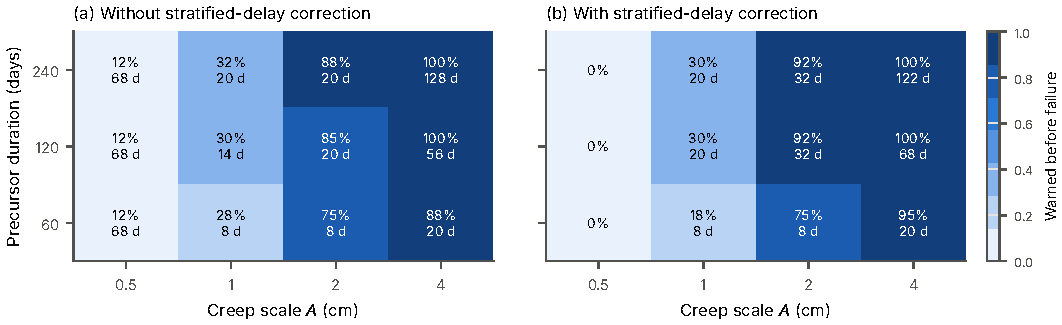
\includegraphics[width=\textwidth]{fig_grid.pdf}
\caption{Share of synthetic failures warned before they occurred (colour, percentage) and median lead time of the warned ones (days), by creep scale $A$ and precursor duration, at the default rule ($k=\PK$, $W=\PWindow$~d, 12-day revisit), (a) without and (b) with the stratified-delay correction. Chance warning rates on matched no-creep scenes: \Chance{} (a) and \ChanceCor{} (b). \Seeds{} realizations per cell.}
\label{fig:grid}
\end{figure*}

\begin{table*}[t]
\caption{Simulation results by creep scale $A$ and precursor duration. Total creep and mid-precursor velocity follow from Eq.~(\ref{eq:creep}). Warned: share of failures warned before they occurred, with Wilson 95\% interval. Lead: median (interquartile range) in days. Default rule; \Seeds{} realizations per row.}
\label{tab:grid}
\begin{ruledtabular}
\begin{tabular}{cccccccc}
 & & & & \multicolumn{2}{c}{Without correction} & \multicolumn{2}{c}{With correction} \\
$A$ (cm) & Precursor (d) & Total creep (cm) & $v$ at mid-precursor (cm/yr) & Warned (\%) & Lead (d) & Warned (\%) & Lead (d) \\
\hline
% Generated by code/09_preprint_numbers.py. Do not edit by hand.
0.5 & 60 & 1.4 & 5.4 & 12 (5--26) & 68 (44--80) & 0 & -- \\
0.5 & 120 & 1.7 & 2.9 & 12 (5--26) & 68 (44--80) & 0 & -- \\
0.5 & 240 & 2.1 & 1.5 & 12 (5--26) & 68 (44--80) & 0 & -- \\
\hline
1 & 60 & 2.8 & 10.7 & 28 (16--43) & 8 (8--56) & 18 & 8 (8--8) \\
1 & 120 & 3.4 & 5.7 & 30 (18--45) & 14 (8--50) & 30 & 20 (8--20) \\
1 & 240 & 4.1 & 2.9 & 32 (20--48) & 20 (8--68) & 30 & 20 (8--20) \\
\hline
2 & 60 & 5.5 & 21.5 & 75 (60--86) & 8 (8--20) & 75 & 8 (8--20) \\
2 & 120 & 6.9 & 11.4 & 85 (71--93) & 20 (8--32) & 92 & 32 (20--44) \\
2 & 240 & 8.2 & 5.9 & 88 (74--95) & 20 (20--56) & 92 & 32 (20--44) \\
\hline
4 & 60 & 11.1 & 43.0 & 88 (74--95) & 20 (20--20) & 95 & 20 (20--20) \\
4 & 120 & 13.7 & 22.8 & 100 (91--100) & 56 (56--68) & 100 & 68 (56--68) \\
4 & 240 & 16.4 & 11.8 & 100 (91--100) & 128 (104--164) & 100 & 122 (116--152) \\

\end{tabular}
\end{ruledtabular}
\end{table*}

\subsection{The threshold trade-off}

Lowering the threshold multiplier raises the warning rate, but it raises the chance rate faster (Fig.~\ref{fig:tradeoff}, Table~\ref{tab:k}). Pooled over all creep settings, $k=2$ warned \KWTwo{} of failures, but its chance rate on no-creep scenes was \KChanceTwo{}, with \KFATwo{} alerts per wall-year. At $k=4$ the chance rate was \KChanceFour{} and the warning rate \KWFour. The default $k=3$ sits at the knee of the curve. Most of the apparent gain from smaller $k$ is coincidence. Of the \KWarnedTwo{} warnings at $k=2$ (out of \KNGrid{} scenes), \KPreTwo{} were raised before the creep had even begun, against \KPreThree{} of \KWarnedThree{} at $k=3$. With the stratified-delay correction the curve moves to the left: the chance rate is \KChanceThreeCor{} at $k=3$ and \KChanceTwoCor{} even at $k=2$, so lower thresholds become usable.

\begin{figure}[t]
\centering
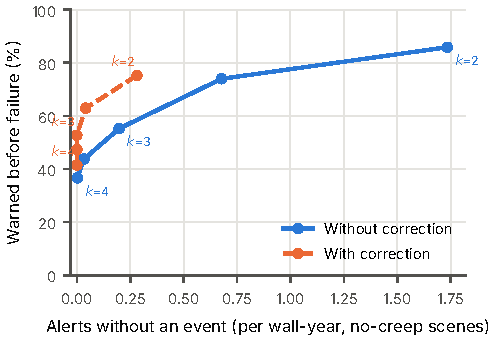
\includegraphics[width=\columnwidth]{fig_tradeoff.pdf}
\caption{Warning rate (all creep settings pooled) against alerts without an event on no-creep scenes, as the threshold multiplier $k$ (labels) varies, without and with the stratified-delay correction.}
\label{fig:tradeoff}
\end{figure}

\begin{table}[t]
\caption{Threshold multiplier $k$: warning rate pooled over all creep settings, chance warning rate and alerts per wall-year on no-creep scenes.}
\label{tab:k}
\begin{ruledtabular}
\begin{tabular}{ccccccc}
 & \multicolumn{3}{c}{Without correction} & \multicolumn{3}{c}{With correction} \\
$k$ & Warned & Chance & /wall-yr & Warned & Chance & /wall-yr \\
\hline
% Generated by code/09_preprint_numbers.py. Do not edit by hand.
2 & 86\% & 68\% & 1.73 & 75\% & 12\% & 0.28 \\
2.5 & 74\% & 42\% & 0.68 & 63\% & 0\% & 0.04 \\
3 & 55\% & 10\% & 0.20 & 53\% & 0\% & 0.00 \\
3.5 & 44\% & 5\% & 0.03 & 47\% & 0\% & 0.00 \\
4 & 37\% & 0\% & 0.00 & 41\% & 0\% & 0.00 \\

\end{tabular}
\end{ruledtabular}
\end{table}

\subsection{Depth-correlated atmosphere drives false alerts}

The dominant source of alerts without an event is the stratified seasonal delay, not the turbulent screen (Fig.~\ref{fig:null}). With $c=0$, no-creep scenes produced \NullZero{} alerts per wall-year at $k=3$. With $c=1.2$, $2.4$ and $4.8$~mm per 100~m of depth the rate rose to \NullOne, \NullTwo{} and \NullFour. Raising $k$ does not help at large $c$, because the seasonal signal is coherent over the whole wall and grows with depth, while the threshold of Eq.~(\ref{eq:thr}) scales with the stable-ground noise, which the seasonal term does not affect. The stratified-delay fit of Eq.~(\ref{eq:strat}) reduced the rates to \NullZeroCor, \NullOneCor, \NullTwoCor{} and \NullFourCor{} per wall-year: \NullUnmatchedCor{} alerts in \NullWallYearsCor{} simulated wall-years at $k=3$.

\begin{figure}[t]
\centering
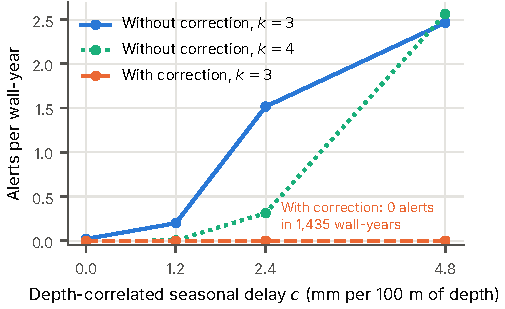
\includegraphics[width=\columnwidth]{fig_null.pdf}
\caption{Alerts without an event per wall-year on no-creep scenes versus the strength of the depth-correlated seasonal delay, without correction ($k=3$ and $k=4$) and with the stratified-delay correction ($k=3$).}
\label{fig:null}
\end{figure}

The same mechanism reverses three intuitive improvements (Table~\ref{tab:variants}). Without correction, a longer velocity window ($W=120$~days), a 6-day revisit, or a quieter turbulent atmosphere each lowers $\sigma_t$ and appears to raise the warning rate for $A=1$~cm creep. In each case, however, the chance rate jumps to \ChanceWinOneTwoZero, \ChanceSix{} and \ChanceAtmTwo, respectively, because the lower threshold now admits the seasonal signal. With the correction, the chance rates are \ChanceWinOneTwoZeroCor, \ChanceSixCor{} and \ChanceAtmTwoCor, and the warning rates are \WWinOneTwoZeroCor, \WSixCor{} and \WAtmTwoCor. Conversely, a noisier atmosphere ($\sigma_{\rm atm}=8$~mm) or a short window ($W=48$~days) suppresses chance alerts and real warnings alike.

\begin{table*}[t]
\caption{Effect of the velocity window, revisit and turbulent-atmosphere strength, without and with the stratified-delay correction. Noise: median stable-ground $\sigma_t$. Chance and alerts per wall-year from matched no-creep scenes. Warned: creep scale 1~cm, 120-day precursor. \Seeds{} realizations per entry.}
\label{tab:variants}
\begin{ruledtabular}
\begin{tabular}{lccccccc}
 & & \multicolumn{3}{c}{Without correction} & \multicolumn{3}{c}{With correction} \\
Setting & Noise (cm/yr) & Chance & Alerts/wall-yr & Warned & Chance & Alerts/wall-yr & Warned \\
\hline
% Generated by code/09_preprint_numbers.py. Do not edit by hand.
Baseline (12 d, 72 d, 4 mm) & 3.5 & 10\% & 0.20 & 30\% & 0\% & 0.00 & 30\% \\
Window 48 d & 6.6 & 5\% & 0.03 & 5\% & 0\% & 0.00 & 5\% \\
Window 120 d & 1.6 & 65\% & 1.42 & 85\% & 0\% & 0.00 & 85\% \\
Revisit 6 d & 2.4 & 62\% & 1.28 & 92\% & 0\% & 0.01 & 95\% \\
Turbulence 2 mm & 2.0 & 57\% & 1.21 & 95\% & 0\% & 0.00 & 92\% \\
Turbulence 8 mm & 6.8 & 2\% & 0.07 & 2\% & 0\% & 0.01 & 5\% \\

\end{tabular}
\end{ruledtabular}
\end{table*}

\subsection{A worked example}

Figure~\ref{fig:example} shows one realization with $A=2$~cm and a 120-day precursor at the default settings. The recovered patch displacement follows the simulated truth until coherence is lost in the final revisits, illustrating Sec.~\ref{sec:alias}. The fastest patch on the east wall crosses the threshold, and an alert is raised \ExampleLead{}~days before failure. The north and south walls, which never move, raised \ExampleNorthAlerts{} and \ExampleSouthAlerts{} short alert episodes over three years. These are the depth-correlated seasonal alerts quantified above, and they are the alerts an analyst would have to dismiss. The hidden west wall contributed no valid pixels in any realization, as intended (maximum \HiddenPx).

\begin{figure}[t]
\centering
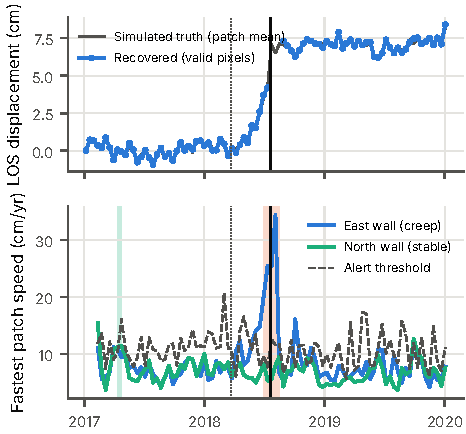
\includegraphics[width=\columnwidth]{fig_example.pdf}
\caption{One synthetic realization ($A=2$~cm, 120-day precursor, default rule). Top: simulated and recovered LOS displacement of the creep patch. Bottom: fastest wall-patch speed for the creeping east wall and the stable north wall, against the alert threshold; shading marks alert episodes on these two walls (orange: east; green: north). Solid line: failure; dotted: creep onset.}
\label{fig:example}
\end{figure}

%=====================================================================
\section{Discussion}\label{sec:discussion}
%=====================================================================

\subsection{What free standardized InSAR can and cannot do for pit walls}

The results bound the role of DISP-S1 to screening, not alarm. A 12-day revisit, a recordable-velocity ceiling of about \AliasTwelve{}~cm/yr, and a lead time measured in revisits make it unsuitable for imminent-collapse warning, which remains the domain of on-site radar and prisms~\cite{Dick2015,Carla2017}. Within that role it is informative. Accelerating creep totalling 5 to 16~cm over two to eight months is flagged before failure in most simulated scenes, at a chance rate near \Chance{} without correction and near zero with it. Equally useful, the product can say in advance which walls it cannot watch, because visibility is a deterministic function of wall orientation, slope and swath position (Sec.~\ref{sec:geom}). A screening program can therefore report three classes of wall: watched and quiet, watched and moving, and unwatchable from this product.

The simulations also argue for a specific processing choice. Thresholds referenced to the noise of stable rim ground are blind to atmospheric delay that tracks pit depth. Whenever random noise is low, through a long window, a dense revisit or calm weather, that delay becomes the main source of alerts. A per-date elevation regression removed the effect in simulation without losing real warnings, and it made the more sensitive settings usable: with a 6-day revisit, \WSixCor{} of failures preceded by 1~cm-scale creep were warned, at a chance rate of \ChanceSixCor. The synthetic seasonal delay was exactly linear in depth, however, so this is an upper bound on the benefit. Real stratification is only approximately linear, mixes with turbulence, and can be compensated by weather models~\cite{Doin2009}. The pilot will therefore report results with and without the correction.

\subsection{Testable expectations for the pilot}

Stating expectations before the real data are analysed makes the pilot a test rather than a demonstration. From Secs.~\ref{sec:geom} and \ref{sec:alias}, we expect the following. (1) The Continental Pit D East highwall will be observable from descending tracks with high LOS sensitivity, and largely unobservable or in layover from ascending tracks, depending on swath position. (2) If the September--October 2022 instability reported by the operator exceeded roughly 1~cm per month of downslope motion (about three times the stable-ground noise of the default 72-day window), the descending record will show an alert before 1 November 2022. If the motion was faster than about \AliasTwelve{}~cm/yr in LOS, the final weeks will appear as coherence loss rather than displacement. (3) The Saga north wall will be recorded at about \SagaMid{} of its downslope motion from either pass, so detection requires roughly twice the downslope speed. Snow cover in late 2022 and January 2023 is likely to remove the final weeks, consistent with the commercial back-analysis~\cite{Bourgeois2024}. Detection of the July--November 2022 crest movement in DISP-S1 would indicate that the free product reproduces the commercial result. Absence of detection would quantify what standardized 30~m processing loses. (4) Alerts without a reported event are expected on deep walls in late summer and winter if the stratified-delay correction is off. Each will be reported and, where possible, explained.

\subsection{Implications for public screening and NISAR}

If the pilot confirms these expectations, a national screen of large US open pits with this pipeline is feasible at no data cost. The screen would produce a per-wall visibility table, which is useful even before any movement is found, together with alerts for analyst review. Two developments should strengthen it: the 6-day revisit restored by Sentinel-1C, provided the depth-correlated delay is corrected (Table~\ref{tab:variants}), and NISAR L-band, whose aliasing ceiling is \AliasRatio{} times higher and whose longer wavelength keeps coherence better on disturbed surfaces. The planned NISAR comparison will repeat the same analysis with the second sensor, using the same code.

%=====================================================================
\section{Limitations}\label{sec:limits}
%=====================================================================

The principal limitations are as follows. (i) No real-data results are reported here. The simulations test the method and the software under controlled assumptions, not the behaviour of real walls. (ii) The synthetic scene is idealized: one conical pit, a planar creep patch, linear depth-correlated delay, and no active mining. In real pits, blasting and loading destroy coherence, and the pipeline cannot distinguish mining from instability. (iii) The geometric analysis uses a planar-slope approximation, typical headings and an assumed $45^\circ$ overall slope for the pilot walls. Actual frames, incidence angles and slopes will be taken from DISP-S1-STATIC and the DEM. (iv) Automatic walls come from a DEM acquired about 2011--2015 and may miss later pushbacks. (v) The stratified-delay fit can absorb part of a large, depth-aligned deformation signal. (vi) Public failure records are incomplete and rarely locate the failure on the wall, so alerts without a reported event are not false alarms, and some events may be unlocated. (vii) Two pits give few events. The pilot will establish feasibility and failure modes, not a national accuracy figure, and its rates will carry wide intervals. (viii) Results apply to DISP-S1 version 1 as downloaded on the dates in the provenance log.

%=====================================================================
\section{Concluding remarks}\label{sec:conclusions}
%=====================================================================

We have built and tested an open pipeline that turns NASA's standardized OPERA DISP-S1 product into wall-by-wall screening of open pits, and we have established what the product can and cannot see before applying it to real failures. Geometry alone decides whether a wall is watchable: with both Sentinel-1 passes, all facing directions of a $45^\circ$ wall are visible and \GeoSensEitherFortyFive{} record at least half of a downslope slide, but steep walls are increasingly hidden. Phase aliasing limits recordable LOS motion to about \AliasTwelve{}~cm/yr at a 12-day revisit. In simulation, the default rule warned of 2~cm-scale accelerating creep in \WTwoOneTwenty{} of scenes, at a chance rate of \Chance, while 0.5~cm-scale creep was indistinguishable from chance. Atmospheric delay that tracks pit depth is the main obstacle to more sensitive settings. An elevation regression removed it in simulation and raised the warning rate to \WTwoOneTwentyCor{}, although its real-world benefit will be smaller than in this idealized test. The two-site pilot will test these predictions against documented failures at the Continental Pit and the Saga Pit, followed by a comparison with NISAR. Every step, from download to this paper's numbers, is public and repeatable, so the method can be checked, criticized and extended by anyone.

\begin{acknowledgments}
OPERA DISP-S1 data are provided by NASA/JPL-Caltech and distributed by the Alaska Satellite Facility DAAC. This work contains modified Copernicus DEM data (ESA/Airbus). Software engineering, data handling and drafting mechanics were assisted by an AI model (Claude, Anthropic). The authors made the analytic decisions, checked the numbers against the pipeline outputs, and take responsibility for the content. Neither pilot site is operated by L.A.'s current or former employers, and L.A. has no financial relationship with their operators. \textbf{[K.K.\ to confirm his competing-interests statement and contribution before submission.]}
\end{acknowledgments}

\section*{Data and code availability}
Code, configuration, tests and provenance records are available at \url{https://github.com/Lookman1234/opera-pitwall-screen}~\cite{Alabede2026}. The simulation results (\texttt{paper/synthetic\_study.csv}), geometry results (\texttt{paper/geometry.json}) and every number in this paper (\texttt{paper/preprint/numbers.tex}) are regenerated by the scripts in \texttt{code/}.

\bibliography{refs}

\end{document}
